\section{Computational Approach}

\begin{figure}
  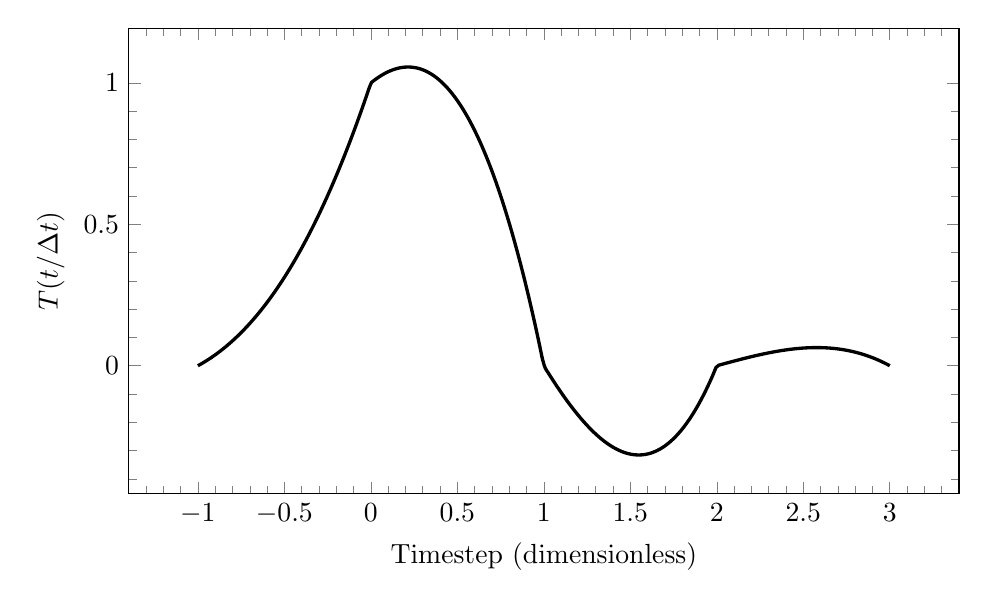
\begin{tikzpicture}[
  declare function = {
    basis(\x) = 
      and(-1 <= \x, \x < 0)*(1+x)*(2+x)*(3+x)/6 +
      and(0  <= \x, \x < 1)*(1-x)*(1+x)*(2+x)/2 +
      and(1  <= \x, \x < 2)*(1-x)*(2-x)*(1+x)/2 + 
      and(2  <= \x, \x < 3)*(1-x)*(2-x)*(3-x)/6 + 
      or(\x <-1, \x > 3)*0;
  }
  ]

  \begin{axis}[width=\columnwidth, height=0.61803398875\columnwidth,
      %xtick={-4, -3, -2, -1},
      minor x tick num={4},
      minor y tick num={4},
      xlabel = Timestep (dimensionless),
      ylabel = {$T(t/\Delta t)$}
      %xticklabels={$-4\Delta t$, $-3\Delta t$, $-2\Delta t$, $-\Delta t$}
  ]
  
  \addplot[very thick, domain=-1:3, smooth, samples=256] {basis(x)};
  \end{axis}
\end{tikzpicture}

  \caption{\label{fig:interpolation basis} Nonorthogonal and $C^0$-continuous temporal basis function $T(t)$ constructed from intervals of fourth-order Lagrange polynomials.}
\end{figure}
To solve \cref{eq:rotating liouville,eq:radiated envelope} for each of $N_s$ \qds{} at $N_t$ equally-spaced timesteps, we begin with a suitable representation of $\tilde{\vb{P}}(\vb{r}, t)$ in terms of spatial and temporal basis functions, i.e.~
\begin{equation}
  \tilde{\vb{P}}(\vb{r}, t) = \sum_{\ell=0}^{N_s - 1} \sum_{m = 0}^{N_t - 1} \alpha_{\ell m} \vb{S}_\ell(\vb{r}) T_m(t)
  \label{eq:basis function representation}
\end{equation}
with $T_m(t) \equiv T(t - m \, \Delta t)$.
As the wavelength of any radiation in the system far exceeds the dimensions of the \qds{} under consideration, we take $\vb{S}_\ell(\vb{r}) \equiv \vb{d}_\ell \delta(\vb{r} - \vb{r}_\ell)$.
Such a discretization additionally discretizes \cref{eq:rotating liouville}, forming a set of $N_s$ first-order differential equations coupled through radiative processes.
Furthermore, we require the $T_m(t)$ to have finite support as well as causal and interpolatory properties so as to recover $\tilde{\vb{P}}$, $\partial_t \tilde{\vb{P}}$, and $\partial^2_t \tilde{\vb{P}}$ at the current timestep.
Accordingly, we have elected to use a set of backwards-looking Lagrange polynomials of order $\ge 4$, forming temporal basis functions similar to the one shown in \cref{fig:interpolation basis}.
These functions  reliably interpolate smooth functions with controllable error and have a long history of use in studies of electromagnetic systems~\cite{SHANKER,SHANKER,SHANKER}.
Combining \cref{eq:radiated envelope,eq:basis function representation} and projecting the resulting field onto the $\vb{S}_\ell$ and $T_m$ basis functions produces a marching-on-in-time system of the form
\begin{equation}
  \sum_{m = 0}^{k} \mathcal{Z}^{(m)} \mathcal{A}^{(k - m)} = \mathcal{F}^{(k)}.
  \label{eq:zmatrix}
\end{equation}
In this (block) matrix equation, $\mathcal{A}^{(k)}$ denotes the (spatial) collection of $\alpha_{\ell k}$ and
\begin{subequations}
  \begin{align}
    \mathcal{Z}^{(m)}_{ij} &= \big\langle \mathbf{S}_i(\vb{r}), \tilde{\mathfrak{F}}\{ \mathbf{S}_j(\mathbf{r}) T(m \, \Delta t) \} \big\rangle \\
    \mathcal{F}^{(k)}_m &= \big\langle \mathbf{S}_m(\vb{r}), \tilde{\mathbf{E}}(\vb{r}, k \, \Delta t) - \tilde{\mathbf{E}}_0(\vb{r}, k \, \Delta t) \big\rangle.
  \end{align}
  \label{eq:projections}
\end{subequations}
As $\mathcal{Z}$ represents a block Toeplitz and lower triangular matrix, \cref{eq:zmatrix} provides a means of calculating $\mathcal{F}^{(k)}$ given only $\mathcal{A}^{(k' \le k)}$.

To link $\mathcal{A}^{(k)}$ with the density matrix in \cref{eq:rotating liouville}, we take
\begin{equation}
  \alpha_{\ell m} \equiv \tilde{\rho}_{01}^{(\ell)}(t = m \, \Delta t)
  \label{eq:polarization definition}
\end{equation}
as the off-diagonal matrix elements (coherences) of $\tilde{\rho}^{(\ell)}$ characterize the dipole radiating at $\vb{r}_\ell$.
Consequently, determining $\mathcal{A}^{(k + 1)}$ amounts to integrating \cref{eq:rotating liouville} from $t = k \, \Delta t$ to $t = \qty(k + 1) \, \Delta t$.
For this, we make use of the predictor/corrector scheme detailed in~\cite{Glaser2009}.
Approximating $\tilde{\rho}(t)$ as a weighted sum of complex exponentials, the predictor/corrector scheme proceeds with an extrapolation predictor step,
\begin{equation}
  \tilde{\rho}(t_{k + 1}) \leftarrow \sum_{\ell = 1}^k \mathcal{P}_\ell^{\qty(0)} \tilde{\rho}(t_\ell) + \mathcal{P}_\ell^{\qty(1)} \dot{\tilde{\rho}}(t_\ell),
  \label{eq:predictor}
\end{equation}
and several iterated corrector steps,
\begin{equation}
  \tilde{\rho}(t_{k + 1}) \leftarrow \mathcal{C}_{k+1}^{\qty(1)} \dot{\tilde{\rho}}(t_{k + 1}) + \sum_{\ell = 1}^k \mathcal{C}_\ell^{\qty(0)} \tilde{\rho}(t) + \mathcal{C}_\ell^{\qty(1)} \dot{\tilde{\rho}}(t_\ell).
  \label{eq:corrector}
\end{equation}
where the $\mathcal{P}_\ell^{\qty(0, 1)}$ and $\mathcal{C}_\ell^{\qty(0, 1)}$ coefficients arise from a least-squares solution to a system of complex-valued exponentials on a semidisk in the left complex plane.
